\chapter{Planificación del proyecto}\label{chap:planif}
La planificación de un proyecto es fundamental para su correcto funcionamiento y
desarrollo, dentro de los plazos y costes establecidos. Se presenta un primer
apartado de metodología, un segundo apartado con la planificación inicial para
posteriormente inferir en base a esta el presupuesto.


\section{Metodología}\label{sec:metodología}
En este capítulo se aborda la metodología adoptada para el desarrollo del
proyecto, fundamentada en principios ágiles y enfocada en la entrega continua de
valor. La elección de \textit{Scrum}, una metodología que permite elaborar
productos software de manera incremental, revisando el producto continuamente y
adaptándolo a las necesidades del cliente, subraya el compromiso con la
adaptabilidad y la mejora continua del producto.

La estructura de este capítulo se organiza en torno a la descripción detallada
de la metodología \textit{Scrum}, la visualización de la planificación y las
estrategias de comunicación adoptadas. A través de esta metodología, se busca
optimizar los recursos disponibles, ajustarse a los plazos establecidos y
garantizar la calidad del producto final.

La implementación de \textit{Scrum} se complementa con herramientas de
visualización y gestión de proyectos, como los tableros \textit{Kanban}, que
facilitan la organización y seguimiento de las tareas. Además, se pone especial
énfasis en la comunicación efectiva dentro del equipo de desarrollo y con los
stakeholders, asegurando así una alineación constante con los objetivos del
proyecto.

Existen otras variantes de los tableros \textit{Kanban} que se pueden
utilizar para visualizar el progreso de las tareas, pero en este proyecto se ha
elegido esta alternativa para facilitar la visualización de las tareas y su
estado~(ver \fullref{subsec:visual_planif}). La visualización de la
planificación es esencial para el seguimiento y control del proyecto, ya que
permite identificar posibles desviaciones y tomar medidas correctivas de manera
temprana.

Este enfoque metodológico no solo refleja la planificación y ejecución del
proyecto, sino que también establece las bases para una gestión eficaz,
adaptativa y orientada a resultados.


\newpage{}
\subsection{Scrum}\label{subsec:scrum}
Para la planificación del proyecto se ha escogido \textit{Scrum}, una
metodología ``ágil'' que se basa en la realización de iteraciones cortas y en la
adaptación a los cambios. La metodología \textit{Scrum} se estructura en
\textit{sprints} (iteraciones cortas de una duración fija), en las que se llevan
a cabo una serie de tareas que se han planificado previamente.

El primer paso de la metodología \textit{Scrum} es la creación de un
\textit{product backlog}, una lista ordenada de las tareas a realizar durante el
desarrollo del producto, a partir de los requisitos del sistema, que a su vez
son una versión refinada de los requisitos iniciales del proyecto. A partir de
este \textit{product backlog} se planifican las tareas que se llevarán a cabo en
cada \textit{sprint}, de manera que sea posible cumplir con los objetivos del
proyecto en el tiempo establecido.

A diferencia de metodologías tradicionales o \emph{en cascada}, \textit{Scrum}
permite la adaptación a los cambios y la mejora continua del producto, ya que se
revisa y se adapta en cada \textit{sprint} según las necesidades del cliente y
del equipo de desarrollo. Por otro lado, \textit{Scrum} se diferencia de otras
metodologías ágiles como \textit{XP} en que no se centra tanto en las prácticas
de desarrollo, sino en la gestión del proyecto y en la entrega de valor al
cliente.

\begin{minipage}{\linewidth}
	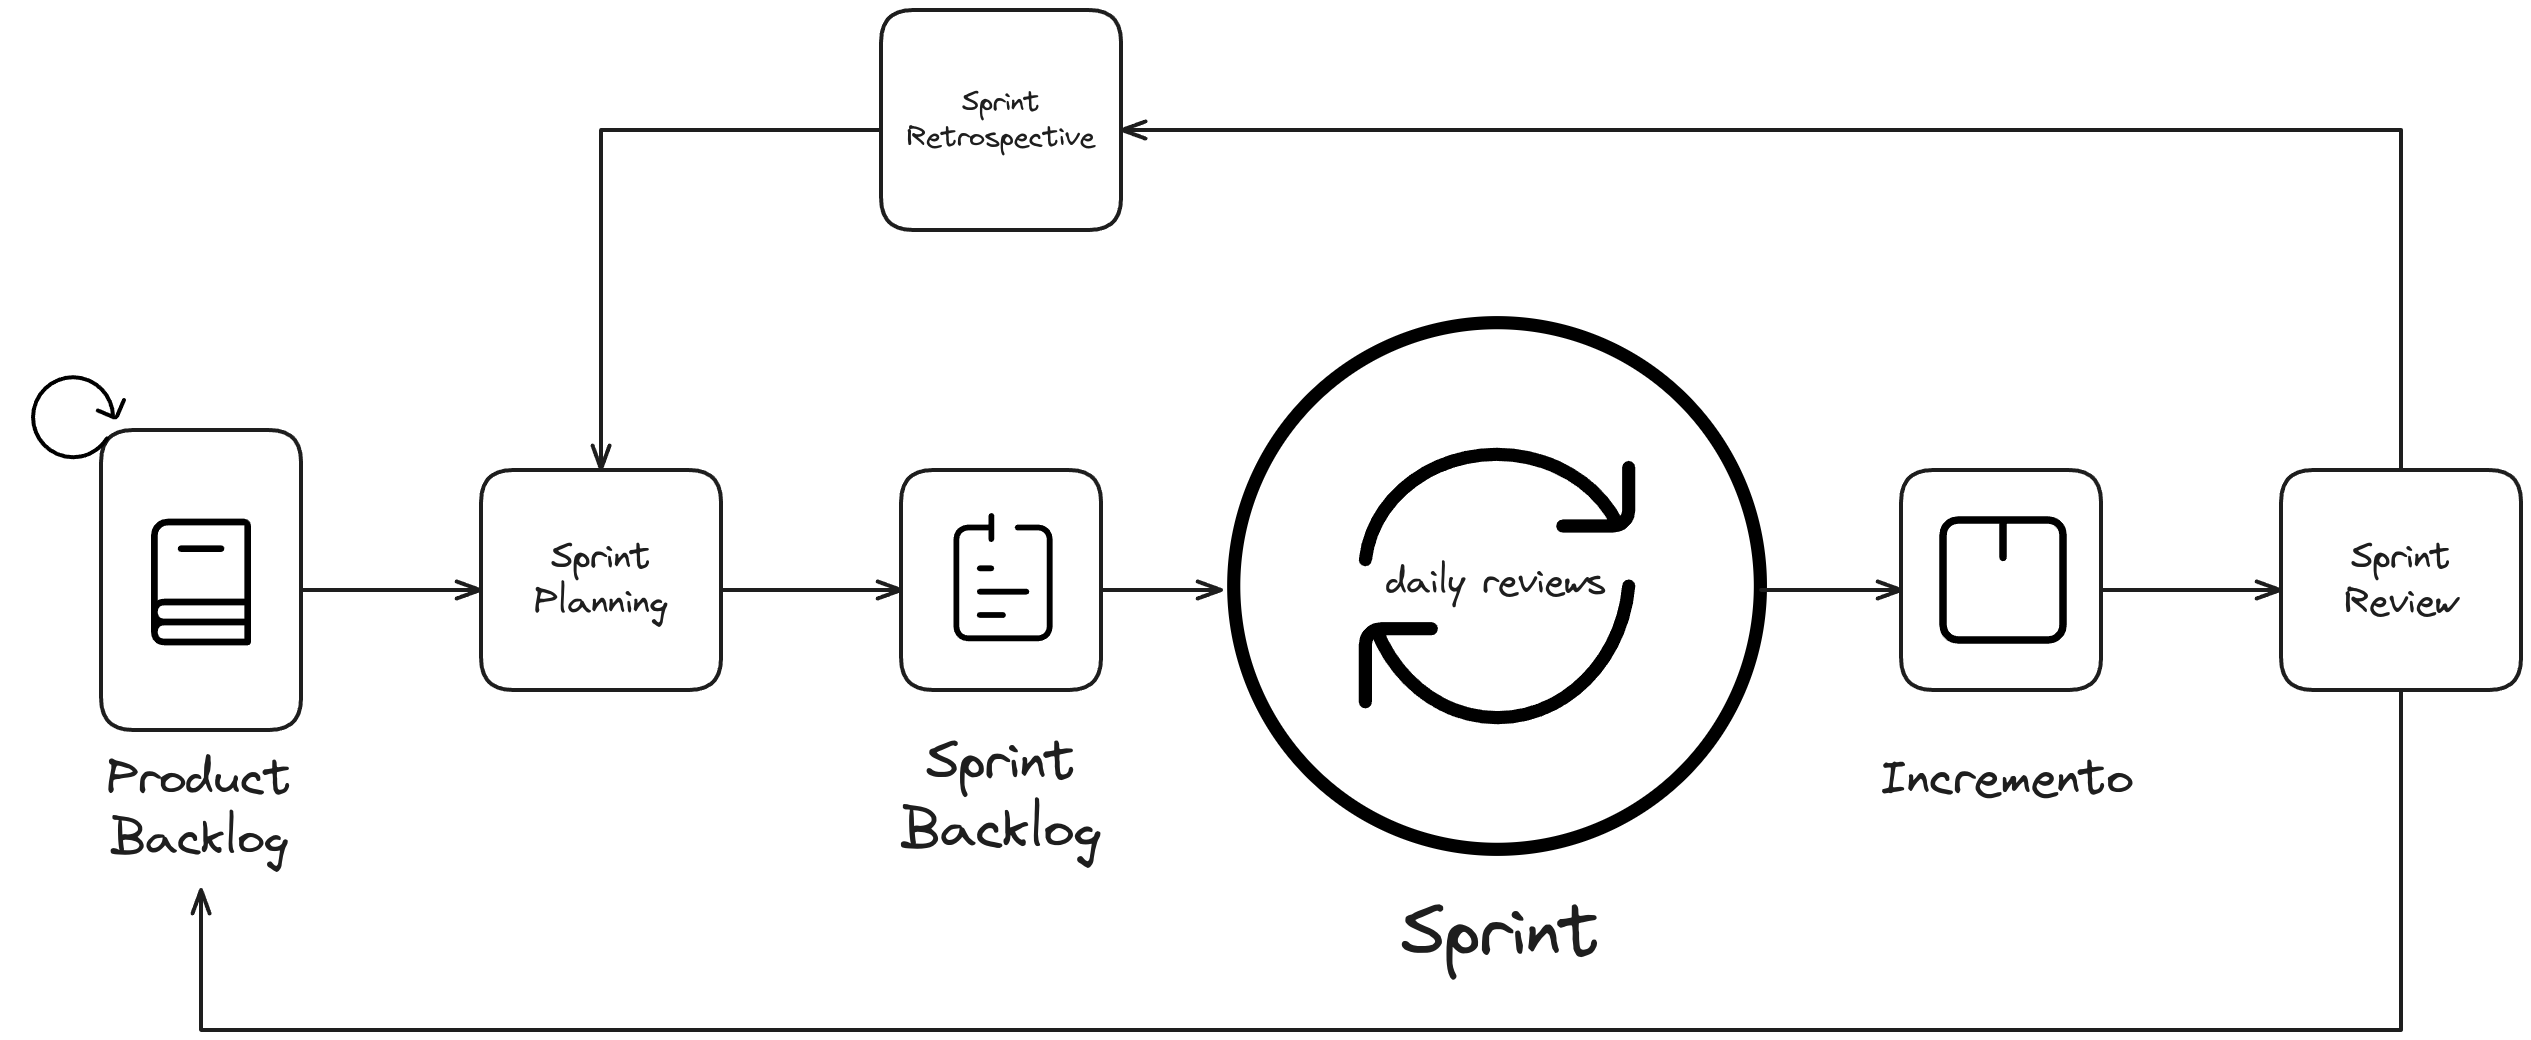
\includegraphics[width=0.85\textwidth]{scrum.png}
	\captionof{figure}{Diagrama de la metodología \textit{Scrum}}
\end{minipage}

\paragraph{Roles}
En \textit{Scrum} se distinguen tres roles principales:

\begin{itemize}
	\item \textbf{Product Owner:} es la persona responsable de definir los
		requisitos del producto y de priorizar las tareas del
		\textit{product backlog}. Es el enlace entre el equipo de desarrollo y
		el cliente, y es el responsable de garantizar que el producto cumple con
		las expectativas del cliente. En el caso de este proyecto, el
		\textit{Product Owner} es el director tecnológico de la empresa.
	\item \textbf{Scrum Master:} es la persona responsable de garantizar que el
		equipo de desarrollo sigue la metodología \textit{Scrum} y de eliminar
		los obstáculos que puedan surgir durante el desarrollo del proyecto. El
		\textit{Scrum Master} es el encargado de organizar las reuniones diarias
		y de asegurar que el equipo de desarrollo cumple con los plazos y los
		objetivos del proyecto. En este proyecto, el \textit{Scrum Master} son
		los tutores académicos del proyecto.
	\item \textbf{Equipo de desarrollo:} es el equipo encargado de llevar a cabo
		las tareas del \textit{product backlog} y de entregar el producto final.
		El equipo de desarrollo es autoorganizado y multidisciplinario, y se
		organiza en torno a las tareas que se van a realizar en cada
		\textit{sprint}. Para este proyecto, el ``equipo'' de desarrollo está
		constituido únicamente por el alumno, que se encarga de todas las tareas
		de desarrollo y documentación.
	\item \textbf{Stakeholders:} son las partes interesadas en el proyecto, como
		los clientes, los usuarios finales y los patrocinadores, que desconocen
		el proceso de desarrollo pero tienen un interés en el producto final y
		en su correcto funcionamiento.
\end{itemize}

\paragraph{Estimación}
En la metodología \textit{Scrum} se pueden utilizar diferentes técnicas de
estimación de tareas, como la estimación en puntos de historia, la estimación en
horas o la estimación en tallas de camiseta. En este proyecto se ha optado por
la estimación en tallas de camiseta, que consiste en asignar a cada tarea una
talla que representa su complejidad y su duración. Las tallas de camiseta se
suelen representar con letras (XS, S, M, L, XL), que se pueden traducir a puntos
de historia siguiendo la secuencia de Fibonacci, es decir, $XS = 1$, $S = 2$,
$M = 3$, $L = 5$, $XL = 8$.

La estimación en Scrum es esencial para la planificación de los \textit{sprints}
y para la asignación de tareas al equipo de desarrollo. La estimación en tallas
se considera óptima para este proyecto, ya que permite una estimación rápida y
sencilla de las tareas, al no necesitar una coordinación entre un equipo
completo de desarrollo.

Además de la estimación del tamaño de las tareas, también se realiza una
estimación sobre la \textit{prioridad} de las mismas, que se representa
siguiendo el equivalente de \textit{GitHub} al sistema de colores de semáforo,
donde el rojo (P0) es la máxima prioridad y el verde (P2) la mínima.

\newpage{}
\subsection{Visualización}\label{subsec:visual_planif}
Para la visualización de la planificación se ha utilizado la herramienta de
gestión de proyecto de \textit{GitHub}, que permite múltiples visualizaciones de
tareas e \textit{issues} en tableros separados.

\begin{itemize}
	\item Se utiliza un tablero de \textit{requisitos} al estilo \textit{Kanban}
		para visualizar los requisitos del proyecto y su estado, siguiendo con
		la metodología \textit{Scrum}. Un tablero \textit{Kanban} es una
		herramienta visual que permite gestionar el flujo de trabajo de un
		proyecto por ``sprints'', dividiendo las tareas en columnas y
		moviéndolas de una columna a otra según su estado.

		\begin{figure}[H]
			\centering
			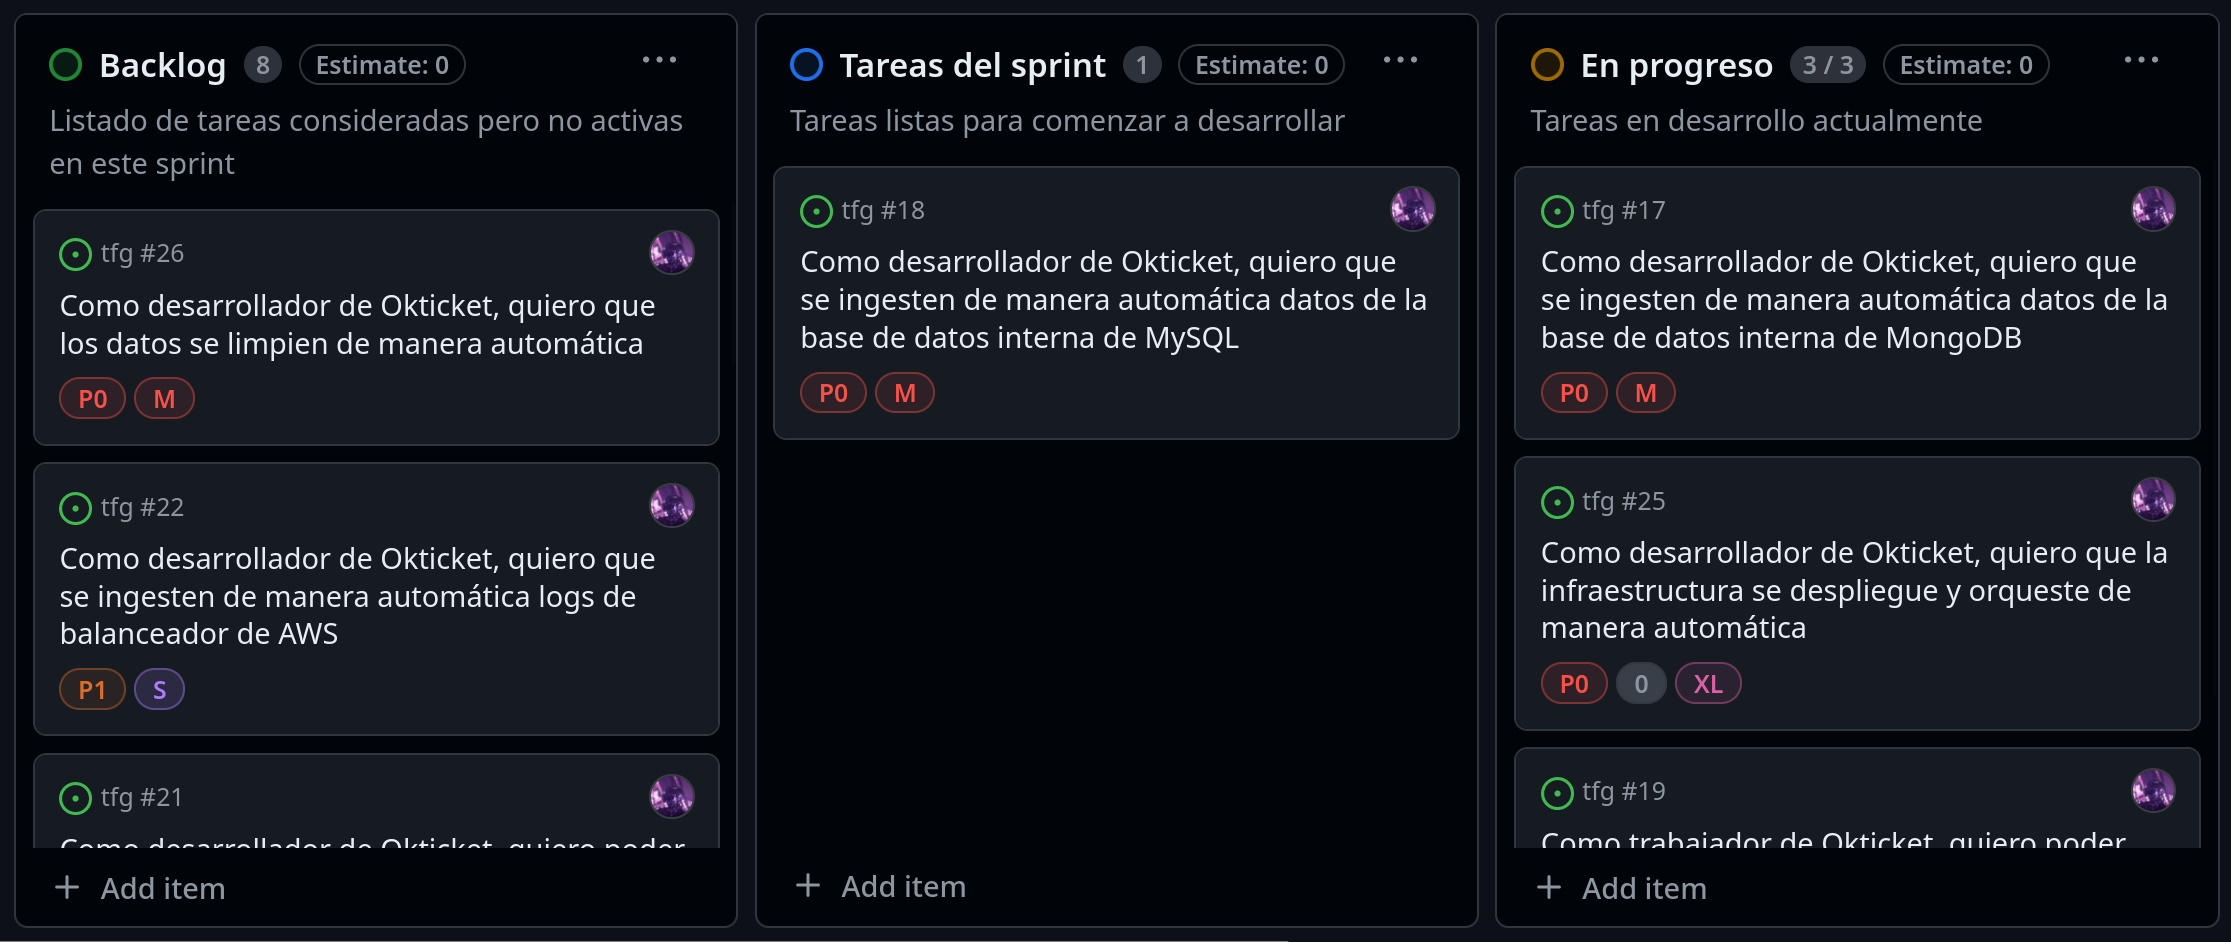
\includegraphics[width=\textwidth]{kanban3.png}
			\caption{Tablero \textit{Kanban} del proyecto}
			\label{fig:kanban}
		\end{figure}
	\item Adicionalmente, se utiliza un \textit{roadmap} de apartados de la
		memoria, separado del tablero de desarrollo normal, donde se visualiza
		su estado y sus fechas límite. Este \textit{roadmap} no está relacionado
		con la metodología \textit{Scrum}, sino que se ha creado para facilitar
		la visualización del progreso de cada sección y de la memoria en general.

		\begin{minipage}{\linewidth}
			\centering
			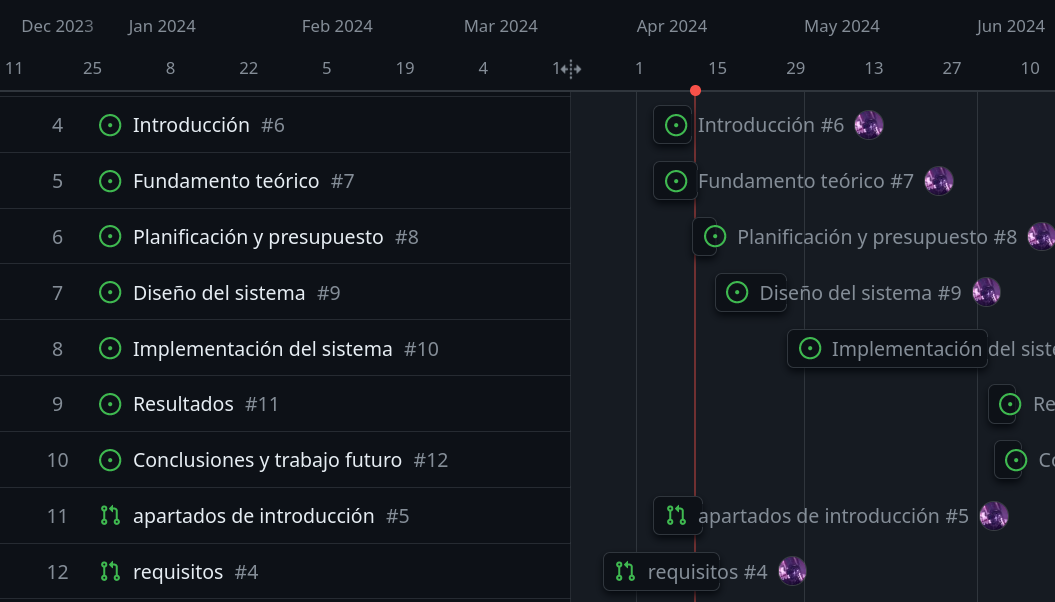
\includegraphics[width=0.9\textwidth]{roadmap.png}
			\captionof{figure}{Roadmap de apartados de la memoria}
		\end{minipage}
\end{itemize}


\subsection{Comunicación}\label{subsec:comunicación}
La comunicación con los tutores y con el equipo de desarrollo se considera
fundamental para el correcto desarrollo del proyecto. Puesto que el trabajo se
desarrolla de manera presencial en la oficina de la empresa, la comunicación con
el equipo de desarrollo se realiza de manera frecuente y directa, mientras que
la comunicación con los tutores se realiza de manera remota pero igual de
frecuente, manteniendo el contacto mediante correo electrónico y Teams para
pedir revisiones e informar sobre el estado del trabajo en todo momento.


\subsection{Herramientas}\label{subsec:herr_planif}
Con el objetivo de facilitar las tareas de desarrollo y cumplimentar los
requisitos por parte de la empresa, se utilizan las siguientes plataformas y
herramientas de desarrollo para la fabricación del proyecto:

\begin{itemize}
	\item \textbf{GitHub:} plataforma de desarrollo colaborativo para el
		desarrollo del proyecto. Se utiliza para la gestión de tareas,
		seguimiento del desarrollo y la documentación del proyecto.
	\item \textbf{Suite de Atlassian (\emph{Jira, Bitbucket}):} Suite de
		herramientas de gestión de proyectos y desarrollo colaborativo. Se
		utiliza para el desarrollo y documentación del proyecto de parte de la
		empresa.
	\item \textbf{Suite de Microsoft (\emph{Teams, Outlook}):} se utilizan las
		plataformas de comunicación puestas a disposición por la universida.
\end{itemize}


\newpage{}
\section{Planificación inicial}\label{sec:planif_inicial}
Como se ha mencionado anteriormente, se utiliza la metodología \textit{Scrum}
para la planificación y desarrollo del proyecto. En la figura \ref{fig:backlog}
se puede ver el \textit{backlog} de tareas que se planifican en el proyecto.

\begin{figure}[H]
	\centering
	
\includegraphics[width=\textwidth]{backlog.png}
	\caption{Planificación inicial del proyecto}
	\label{fig:backlog}
\end{figure}

Las tareas anteriores se clasifican y categorizan según su prioridad y tamaño,
haciendo uso de la estrategia de tallas de camiseta como mencionado
anteriormente. En el tablero \textit{Kanban} (ver figura \ref{fig:kanban}) se
puede ver en todo momento el estado de las tareas, su progreso y sus
características. El listado de tareas iniciales (ordenado según su prioridad)
es el siguiente:

\begin{table}[H]
	\centering
	\begin{tabular}{|p{0.7\linewidth}|c|c|}
		\hline
		\textbf{Tarea} & \textbf{Prioridad} & \textbf{Tamaño} \\
		\hline
		\hline
		Creación de la infraestructura base (técnica) & P0\cellcolor{red!50} & L\cellcolor{orange!50} \\
		\hline
		Como desarrollador de Okticket, quiero que la arquitectura se despliegue y orqueste de manera automática & P0\cellcolor{red!50} & XL\cellcolor{red!50} \\
		\hline
		Como desarrollador de Okticket, quiero que se ingesten de manera automática datos de la base de datos interna de MongoDB & P0\cellcolor{red!50} & M\cellcolor{yellow!50} \\
		\hline
		Como desarrollador de Okticket, quiero que se ingesten de manera automática datos de la base de datos interna de MySQL & P0\cellcolor{red!50} & M\cellcolor{yellow!50} \\
		\hline
		Como desarrollador de Okticket, quiero que los datos se limpien de manera automática & P0\cellcolor{red!50} & M\cellcolor{yellow!50} \\
		\hline
		Como trabajador de Okticket, quiero poder ver y consultar datos internos de la empresa & P1\cellcolor{orange!50} & L\cellcolor{orange!50} \\
		\hline
		Como desarrollador de Okticket, quiero que se ingesten de manera automática logs de balanceador de AWS & P1\cellcolor{orange!50} & S\cellcolor{green!25} \\
		\hline
		Como desarrollador de Okticket, quiero poder ver el estado general de la infraestructura & P1\cellcolor{orange!50} & L\cellcolor{orange!50} \\
		\hline
		Como desarrollador de Okticket, quiero que los datos contengan metadatos que faciliten su filtrado o búsqueda & P2\cellcolor{yellow!50} & S\cellcolor{green!25} \\
		\hline
		Como trabajador de Okticket, quiero poder ver y consultar datos de empresas cliente & P2\cellcolor{yellow!50} & M\cellcolor{yellow!50} \\
		\hline
		Como gestor de una empresa cliente, quiero poder ver información relevante sobre mi empresa que recoja Okticket & P2\cellcolor{yellow!50} & L\cellcolor{orange!50} \\
		\hline
		Como desarrollador de Okticket, quiero poder ingestar datos de APIs externas a la empresa & P2\cellcolor{yellow!50} & L\cellcolor{orange!50} \\
		\hline
		Como desarrollador de Okticket, quiero poder ingestar información de páginas web externas (\textit{scraping}) & P2\cellcolor{yellow!50} & XL\cellcolor{red!50} \\
		\hline
	\end{tabular}
	\caption{Listado de tareas iniciales}
	\label{tab:initial_tasks}
\end{table}

Siguiendo la tabla anterior, se pueden planear los \textit{sprints} y
asignar las tareas a cada uno de ellos.


\newpage{}
\section{Presupuesto}\label{sec:presupuesto}
Para poder llevar a cabo este proyecto, se realiza una estimación del coste
total neceario para su desarrollo, que se divide en dos partes: el coste del
material, que incluye el coste de los recursos necesarios para el desarrollo del
proyecto, y el coste del personal, que incluye el coste de las horas de trabajo
del desarrollador.


\subsection{Presupuesto de material}\label{subsec:pres_material}
Puesto que el proyecto se desarrolla en la empresa, se dispone de todos los
recursos físicos necesarios para llevar a cabo el proyecto, es decir, que no se
incluirá el coste del ordenador o de la conexión a internet en el presupuesto.

Sin embargo, se incluirá el coste de las herramientas y servicios utilizados
durante el desarrollo del proyecto, como el coste de las licencias de software,
el coste de los servicios en la nube, el coste de las herramientas de
desarrollo, etc.

Es importante destacar de que los precios de los servicios en la nube son
aproximados y pueden variar en función de la región, el tipo de instancia, el
tipo de almacenamiento, etc. Por lo tanto, los precios presentados en este
presupuesto son orientativos y pueden variar en función de las necesidades del
proyecto. En este caso, se analizan los precios en junio de 2024 en la región
de Amazon Web Services (AWS) de \textit{eu-west-3} (París).

\begin{table}[H]
	\centering
	\small
	\begin{tabular}{|l|l|r|r|r|}
	\hline
	\textbf{Categoría} & \textbf{Ítem} & \textbf{Cantidad} & \textbf{Coste unitario} & \textbf{Coste total} \\
	\hline
	\hline
	AWS Compute & Fargate & 500 vCPU-h/mes & 0,04665€/vCPU-h & 23,33€ \\
	 & & 1000 GB-h/mes & 0,00511€/GB-h & 5,11€ \\
	\hline
	AWS Storage & EFS & 500 GB/mes & 0,36€/GB-mes & 180,00€ \\
	 & S3 & 250 GB/mes & 0,0245€/GB-mes & 6,13€ \\
	\hline
	AWS Network & VPC & 4 NAT Gateways & 0,052€/h & 149,76€ \\
	 & ELB & 4 ALBs & 0,0243€/h & 70,00€ \\
	\hline
	AWS Security & IAM & - & Sin cargo & 0,00€ \\
	 & KMS & 1 CMK & 1,00€/mes & 1,00€ \\
	\hline
	Stack KELK & Kafka & - & Licencia gratuita & 0,00€ \\
	 & Elasticsearch & - & Licencia gratuita & 0,00€ \\
	 & Logstash & - & Licencia gratuita & 0,00€ \\
	 & Kibana & - & Licencia gratuita & 0,00€ \\
	\hline
	AWS Container & ECS & - & Sin cargo & 0,00€ \\
	\hline
	AWS Monitor & CloudWatch & 5 métricas & 0,30€/métrica-mes & 1,50€ \\
	 & X-Ray & 50,000 trazas/mes & 4,60€/1M trazas & 0,23€ \\
	\hline
	Despliegue & Terraform & - & Licencia gratuita & 0,00€ \\
	\hline
	Capacitación & Cursillo online & 1 & 184,00€ & 184,00€ \\
	\hline
	\textbf{Subtotal} & \multicolumn{4}{r|}{620,06€} \\
	\hline
	\hline
	Otros & Support & Plan Basic & Sin cargo & 0,00€ \\
	 & Optimización & - & 5\% del subtotal & 31,00€ \\
	 & Contingencia & - & 10\% del subtotal & 62,00€ \\
	\hline
	\textbf{Total} & \multicolumn{4}{r|}{713,06€} \\
	\hline
	\end{tabular}
	\caption{Propuesta de presupuesto de materiales}
	\label{tab:presupuesto_material}
\end{table}


\newpage{}
\subsection{Presupuesto de personal}\label{subsec:pres_personal}
A continuación, se presenta una propuesta de presupuesto de personal para el
desarrollo del proyecto, que incluye el coste de las horas de trabajo según
cada rol y el coste total del personal.

\begin{table}[H]
	\centering
	\small
	\begin{tabular}{|l|l|r|r|r|}
	\hline
	\textbf{Rol} & \textbf{Descripción} & \textbf{Horas/mes} & \textbf{CU (€/h)} & \textbf{CT (€/mes)} \\
	\hline
	\hline
	Arquitecto & Diseño de la arquitectura y supervisión & 40 & 60 & 2.400,00€ \\
	\hline
	Desarrollador & Desarrollo y mantenimiento & 160 & 45 & 7.200,00€ \\
	\hline
	Administrador & Gestión de sistemas y seguridad & 160 & 50 & 8.000,00€ \\
	\hline
	DevOps & Infraestructuras y monitorización & 80 & 55 & 4.400,00€ \\
	\hline
	\textbf{Subtotal} & \multicolumn{4}{r|}{22.000,00€} \\
	\hline
	\hline
	Otros & \multicolumn{3}{|l|}{IVA (21\%)} & 4.620,00€ \\
	 & \multicolumn{3}{|l|}{Margen (5\%)} & 1.100,00€ \\
	\hline
	\textbf{Total} & \multicolumn{4}{r|}{27.720,00€} \\
	\hline
	\end{tabular}
	\caption{Propuesta de presupuesto de personal}
	\label{tab:presupuesto_personal_aws}
\end{table}

El coste del personal es ficticio, pero se ha calculado en base a experiencias
previas de contratación y subcontratación de personal en la empresa, además de
tener en cuenta el coste medio de los roles en Asturias.

\subsection{Presupuesto total}\label{subsec:pres_total}
Finalmente, se presenta el presupuesto total del proyecto, que incluye el coste
del material y el coste del personal, así como el coste total del proyecto.

\begin{table}[H]
	\centering
	\small
	\begin{tabular}{|l|r|}
	\hline
	\textbf{Concepto} & \textbf{Coste (€/mes)} \\
	\hline
	Presupuesto de materiales & 713,06€ \\
	\hline
	Presupuesto de personal & 27.720,00€ \\
	\hline
	\textbf{Subtotal} & \textbf{28.433,06€} \\
	\hline
	\hline
	Beneficio Industrial (15\%) & 4.264,96€ \\
	\hline
	\textbf{Total} & \textbf{32.698,02€} \\
	\hline
	\end{tabular}
	\caption{Costes combinados de presupuesto y materiales con beneficio industrial}
	\label{tab:costes_combinados}
\end{table}

El presupuesto total del proyecto asciende a 32.698,02€ (treinta y dos mil
seiscientos noventa y ocho euros con dos céntimos), que incluye el coste del
material, el coste del personal y el beneficio industrial, además de sus
márgenes.
